\section{Composición}

\subsection{Introducción}

El método de Composición se aplica cuando la función de densidad puede dividirse en subfunciones $f_i(x)$ ponderadas por subáreas $A_i$; internamente cada subfunción se resuelve con Transformada Inversa. En este problema se aplica a una distribución triangular simbólica definida por los parámetros $a$, $b$, $c$.

\subsection{Descripción del problema}

\begin{quote}
Se tiene la siguiente distribución triangular en $[a,c]$ con vértice en $b$:
\end{quote}

\begin{center}
\shorthandoff{>}
\begin{tikzpicture}[scale=1.2]
  \draw[->] (0,0) -- (8,0) node[right] {$x$};
  \draw[->] (0,0) -- (0,4) node[above] {$f(x)$};
  \draw (1.5,0) -- (4,3) -- (6.5,0);
  \draw[dashed] (4,0) -- (4,3);
  \node[below] at (1.5,0) {$a$};
  \node[below] at (4,0)   {$b$};
  \node[below] at (6.5,0) {$c$};
\end{tikzpicture}
\shorthandon{>}
\end{center}

\[
f(x)=\begin{cases}
\dfrac{2(x-a)}{(b-a)(c-a)} &;\ a \leq x \leq b \\[8pt]
\dfrac{2(c-x)}{(c-a)(c-b)} &;\ b \leq x \leq c
\end{cases}
\]

\subsection{Propuesta de solución}

Se aplica el método de Composición, que requiere seguir los siguientes pasos.

\textbf{Paso 1: Contar con la función $f(x)$ y dividirla en subáreas}

\[
f(x) = \sum_{i=1}^{n} f_i(x) \cdot A_i \qquad ; \qquad \sum_{i=1}^{n} A_i = 1
\]

Determinando la altura $h$ de modo que $A_1 + A_2 = 1$:
\[
\tfrac{1}{2}(b-a)\cdot h + \tfrac{1}{2}(c-b)\cdot h = 1
\]
\[
\tfrac{h}{2}\big((b-a)+(c-b)\big) = 1
\]
\[
\tfrac{h}{2}(c-a) = 1
\]
\[
h = \frac{2}{c-a}
\]

Determinando subárea $A_1$:
\[
A_1 = \tfrac{1}{2}(b-a)\cdot\frac{2}{c-a} = \frac{b-a}{c-a}
\]

Determinando subárea $A_2$:
\[
A_2 = \tfrac{1}{2}(c-b)\cdot\frac{2}{c-a} = \frac{c-b}{c-a}
\]

\textbf{Paso 2: Definir las subfunciones $f_i(x)$}

Para la 1ra parte ($A_1'=1$), definida por los puntos $(a,0)$ y $(b,h_1)$:
\[
A_1' = \tfrac{1}{2}(b-a)\,h_1 = 1 \implies h_1 = \frac{2}{b-a}
\]
Ecuación de la recta:
\[
\frac{y - 0}{\dfrac{2}{b-a} - 0} = \frac{x - a}{b - a}
\]
\[
f_1(x) = \frac{2(x-a)}{(b-a)^2} \qquad ;\ a \leq x \leq b
\]

Para la 2da parte ($A_2'=1$), definida por los puntos $(b,h_2)$ y $(c,0)$:
\[
A_2' = \tfrac{1}{2}(c-b)\,h_2 = 1 \implies h_2 = \frac{2}{c-b}
\]
Ecuación de la recta:
\[
\frac{y - 0}{\dfrac{2}{c-b} - 0} = \frac{x - c}{b - c}
\]
\[
f_2(x) = \frac{-2(x-c)}{(c-b)^2} \qquad ;\ b \leq x \leq c
\]

\textbf{Paso 3: Reexpresar $f(x)$ en términos de $f_i(x)$ y $A_i$}

\[
f(x) = \frac{2(x-a)}{(b-a)^2}\cdot\frac{b-a}{c-a} + \frac{-2(x-c)}{(c-b)^2}\cdot\frac{c-b}{c-a}
\]
\[
f(x) = \frac{2(x-a)}{(b-a)(c-a)} - \frac{2(x-c)}{(c-b)(c-a)}
\]

Verificación: $A_1+A_2 = \dfrac{b-a}{c-a}+\dfrac{c-b}{c-a} = \dfrac{c-a}{c-a} = 1$ \checkmark

\textbf{Paso 4: Generar números aleatorios}

\[
R_1 \leftarrow \text{gcm}() \qquad ; \qquad R_2 \leftarrow \text{gcm}()
\]

\textbf{Paso 5: Relación entre acumuladas de área y subfunciones}

\[
\text{si } R_1 < A_1 = \frac{b-a}{c-a} \implies \text{escoger } f_1(x)
\]
\[
\text{si } R_1 \geq A_1 \implies \text{escoger } f_2(x)
\]

\textbf{Paso 6: Escoger subfunción con $R_1$}

\begin{lstlisting}[caption={Selección de subfunción}, language=Pascal]
si (R1 < (b-a)/(c-a))
    escoger f1(x)
sino
    escoger f2(x)
fin si
\end{lstlisting}

\textbf{Paso 7: Aplicar Transformada Inversa a la subfunción escogida}

\textit{Aplicando TI a la subfunción $f_1(x)$:}

\textbf{Paso 1.} Sea $f_1(x)$:
\[
f_1(x) = \frac{2(x-a)}{(b-a)^2} \qquad ;\ a \leq x \leq b
\]

\textbf{Paso 2.} Determinar la función acumulada $F_1(x)$:
\[
F_1(x) = \int_a^x \frac{2(x-a)}{(b-a)^2}\,dx = \frac{2}{(b-a)^2} \int_a^x (x-a)\,dx
\]
Aplicando la regla de la potencia:
\[
F_1(x) = \frac{2}{(b-a)^2} \left[\frac{(x-a)^2}{2}\right]_a^x = \frac{2}{(b-a)^2}\cdot\frac{(x-a)^2}{2}
\]
\[
\boxed{F_1(x) = \frac{(x-a)^2}{(b-a)^2}} \qquad ;\ a \leq x \leq b
\]

\textbf{Paso 3.} Igualar $F_1(x) = R_2$:
\[
\frac{(x-a)^2}{(b-a)^2} = R_2
\]

\textbf{Paso 4.} Aplicar función inversa:
\[
(x-a)^2 = (b-a)^2\,R_2
\]
\[
x - a = (b-a)\sqrt{R_2}
\]
\[
x_1=\begin{cases}a+(b-a)\sqrt{R_2} &;\ 0 \leq R_2 \leq 1 \\ 0 &;\ 0 > R_2 > 1\end{cases}
\]

\textit{Aplicando TI a la subfunción $f_2(x)$:}

\textbf{Paso 1.} Sea $f_2(x)$:
\[
f_2(x) = \frac{-2(x-c)}{(c-b)^2} \qquad ;\ b \leq x \leq c
\]

\textbf{Paso 2.} Determinar la función acumulada $F_2(x)$:
\[
F_2(x) = \int_b^x \frac{-2(x-c)}{(c-b)^2}\,dx = \frac{-2}{(c-b)^2} \int_b^x (x-c)\,dx
\]
Aplicando la regla de la potencia:
\[
F_2(x) = \frac{-2}{(c-b)^2}\left[\frac{(x-c)^2}{2}\right]_b^x = \frac{-2}{(c-b)^2}\cdot\left(\frac{(x-c)^2}{2} - \frac{(b-c)^2}{2}\right)
\]
Expandiendo $(b-c)^2 = (b-c)(b-c) = b^2-2bc+c^2 = (c-b)^2$:
\[
F_2(x) = \frac{-2}{(c-b)^2}\cdot\frac{(x-c)^2-(c-b)^2}{2} = \frac{-(x-c)^2+(c-b)^2}{(c-b)^2}
\]
\[
\boxed{F_2(x) = 1 - \frac{(x-c)^2}{(c-b)^2}} \qquad ;\ b \leq x \leq c
\]

\textbf{Paso 3.} Igualar $F_2(x) = R_2$:
\[
1 - \frac{(x-c)^2}{(c-b)^2} = R_2 \implies \frac{(x-c)^2}{(c-b)^2} = 1-R_2
\]

\textbf{Paso 4.} Aplicar función inversa:
\[
(x-c)^2 = (c-b)^2(1-R_2)
\]
Como $b \leq x \leq c$ entonces $x-c \leq 0$, se toma la raíz negativa:
\[
x-c = -(c-b)\sqrt{1-R_2}
\]
\[
x_2=\begin{cases}c-(c-b)\sqrt{1-R_2} &;\ 0 \leq R_2 \leq 1 \\ 0 &;\ 0 > R_2 > 1\end{cases}
\]

La variable final por composición:
\[
x=\begin{cases}
x_1 = a+(b-a)\sqrt{R_2}   & ;\ R_1 < \dfrac{b-a}{c-a} \\[8pt]
x_2 = c-(c-b)\sqrt{1-R_2} & ;\ R_1 \geq \dfrac{b-a}{c-a}
\end{cases}
\]

\textbf{Paso 8: Repetir para el tamaño de muestra requerido}

Se repiten los pasos anteriores para generar las observaciones necesarias de la simulación.

\subsection{Objetivos}

\textbf{Objetivo general:} Aplicar el método de Composición (con Transformada Inversa) para generar valores aleatorios de una variable con distribución triangular en $[a,c]$.

\textbf{Objetivos específicos:}
\begin{enumerate}
    \item Determinar las subfunciones $f_1(x)$, $f_2(x)$ y sus subáreas $A_1$, $A_2$ mediante el método de composición.
    \item Validar mediante prueba de escritorio que los valores generados se ajustan al rango $[a,c]$ y a la proporción esperada entre subfunciones.
\end{enumerate}

\subsection{Desarrollo de la solución}

\subsubsection{Algoritmo}

Del modelamiento se obtiene la propuesta algorítmica para generar la variable aleatoria $x$:

\begin{lstlisting}[caption={Pseudocódigo — Método de Composición}, language=Pascal]
FUNCION variableComposicion() : Real
    DEFINIR R1, R2, x : Real
    R1 <- gcm()
    R2 <- gcm()
    SI R1 < (b-a)/(c-a) ENTONCES
        x <- a + (b-a) * raiz(R2)
    SINO
        x <- c - (c-b) * raiz(1-R2)
    FIN SI
    Retornar x
FIN FUNCION
\end{lstlisting}

\subsubsection{Diagrama de flujo}

\begin{figure}[H]
\centering
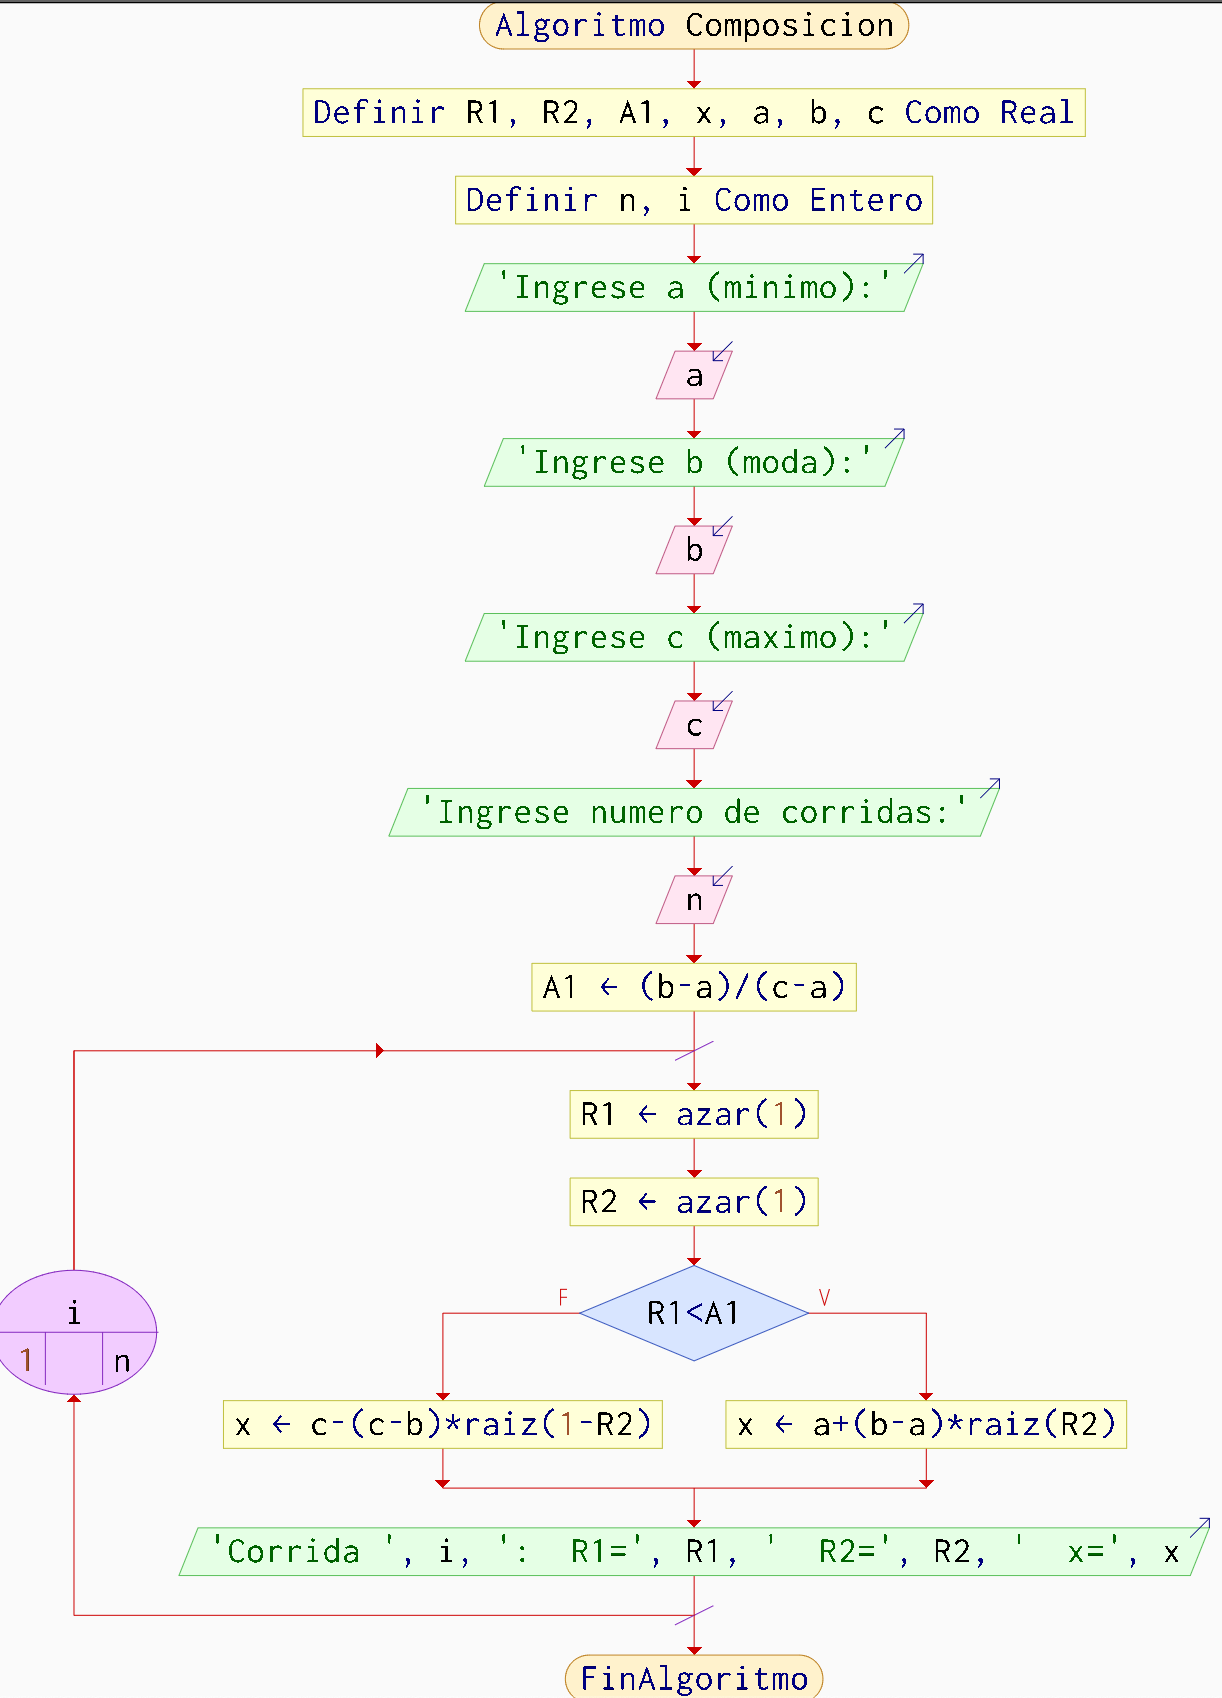
\includegraphics[width=0.5\textwidth]{capturas_pseint/p2_composicion.png}
\caption{Diagrama de flujo — Composición (PSeInt)}
\end{figure}

\subsubsection{Tabla de simulación}

Con $a=1{,}5$, $b=4$, $c=6{,}5$ y $A_1=\dfrac{b-a}{c-a}=0{,}5$.
Cada fila es una corrida; cada columna es un paso del algoritmo:

\begin{mitabla}[H]{Tabla de simulación con $n=10$}
\small
\begin{tabular}{c c c c L{5.5cm}}
\toprule
Corrida & $R_1 \leftarrow \text{gcm}()$ & $R_2 \leftarrow \text{gcm}()$ & Sub & $x$ \\
\midrule
1  & 0,9077 & 0,5115 & $f_2$ & $6{,}5-2{,}5\sqrt{1-0{,}5115}=4{,}7527$ \\
2  & 0,2128 & 0,0785 & $f_1$ & $1{,}5+2{,}5\sqrt{0{,}0785}=2{,}2005$ \\
3  & 0,4475 & 0,7656 & $f_1$ & $1{,}5+2{,}5\sqrt{0{,}7656}=3{,}6875$ \\
4  & 0,6524 & 0,7491 & $f_2$ & $6{,}5-2{,}5\sqrt{1-0{,}7491}=5{,}2478$ \\
5  & 0,4321 & 0,6206 & $f_1$ & $1{,}5+2{,}5\sqrt{0{,}6206}=3{,}4694$ \\
6  & 0,7857 & 0,5601 & $f_2$ & $6{,}5-2{,}5\sqrt{1-0{,}5601}=4{,}8419$ \\
7  & 0,3858 & 0,2163 & $f_1$ & $1{,}5+2{,}5\sqrt{0{,}2163}=2{,}6627$ \\
8  & 0,7241 & 0,1473 & $f_2$ & $6{,}5-2{,}5\sqrt{1-0{,}1473}=4{,}1915$ \\
9  & 0,6775 & 0,1335 & $f_2$ & $6{,}5-2{,}5\sqrt{1-0{,}1335}=4{,}1729$ \\
10 & 0,0111 & 0,2878 & $f_1$ & $1{,}5+2{,}5\sqrt{0{,}2878}=2{,}8411$ \\
\bottomrule
\end{tabular}
\end{mitabla}

\subsubsection{Implementación}

\begin{mitabla}[H]{Variables del modelamiento}
\begin{tabular}{cL{8cm}c}
\toprule
Variable & Descripción & Paso \\
\midrule
$R_1$ & Número aleatorio para seleccionar subfunción, $0 < R_1 < 1$ & Paso 4 \\
$R_2$ & Número aleatorio para aplicar transformada inversa, $0 < R_2 < 1$ & Paso 4 \\
$x$   & Variable generada por composición según $R_1$ & Paso 7 \\
\bottomrule
\end{tabular}
\end{mitabla}

\textbf{Implementación en Java:}

\begin{lstlisting}[caption={Composicion.java}, language=Java]
import java.util.Scanner;

public class Composicion {

    public static double generarX(double a, double b, double c) {
        double R1 = Math.random();
        double R2 = Math.random();
        double A1 = (b - a) / (c - a);
        if (R1 < A1) {
            return a + (b - a) * Math.sqrt(R2);
        } else {
            return c - (c - b) * Math.sqrt(1 - R2);
        }
    }

    public static void main(String[] args) {
        Scanner sc = new Scanner(System.in);
        System.out.print("Ingrese a (minimo): ");  double a = sc.nextDouble();
        System.out.print("Ingrese b (moda):   ");  double b = sc.nextDouble();
        System.out.print("Ingrese c (maximo): ");  double c = sc.nextDouble();
        System.out.print("Ingrese n:          ");  int n = sc.nextInt();

        System.out.println("Corrida\tR1\t\tR2\t\tSubfuncion\tx");
        for (int i = 1; i <= n; i++) {
            double R1 = Math.random();
            double R2 = Math.random();
            double A1 = (b - a) / (c - a);
            double x;  String sub;
            if (R1 < A1) { x = a+(b-a)*Math.sqrt(R2);     sub="f1"; }
            else          { x = c-(c-b)*Math.sqrt(1-R2);   sub="f2"; }
            System.out.printf("%d\t%.4f\t\t%.4f\t\t%s\t\t%.4f%n",i,R1,R2,sub,x);
        }
        sc.close();
    }
}
\end{lstlisting}

\textbf{Implementación en Excel:}

\begin{figure}[H]
\centering
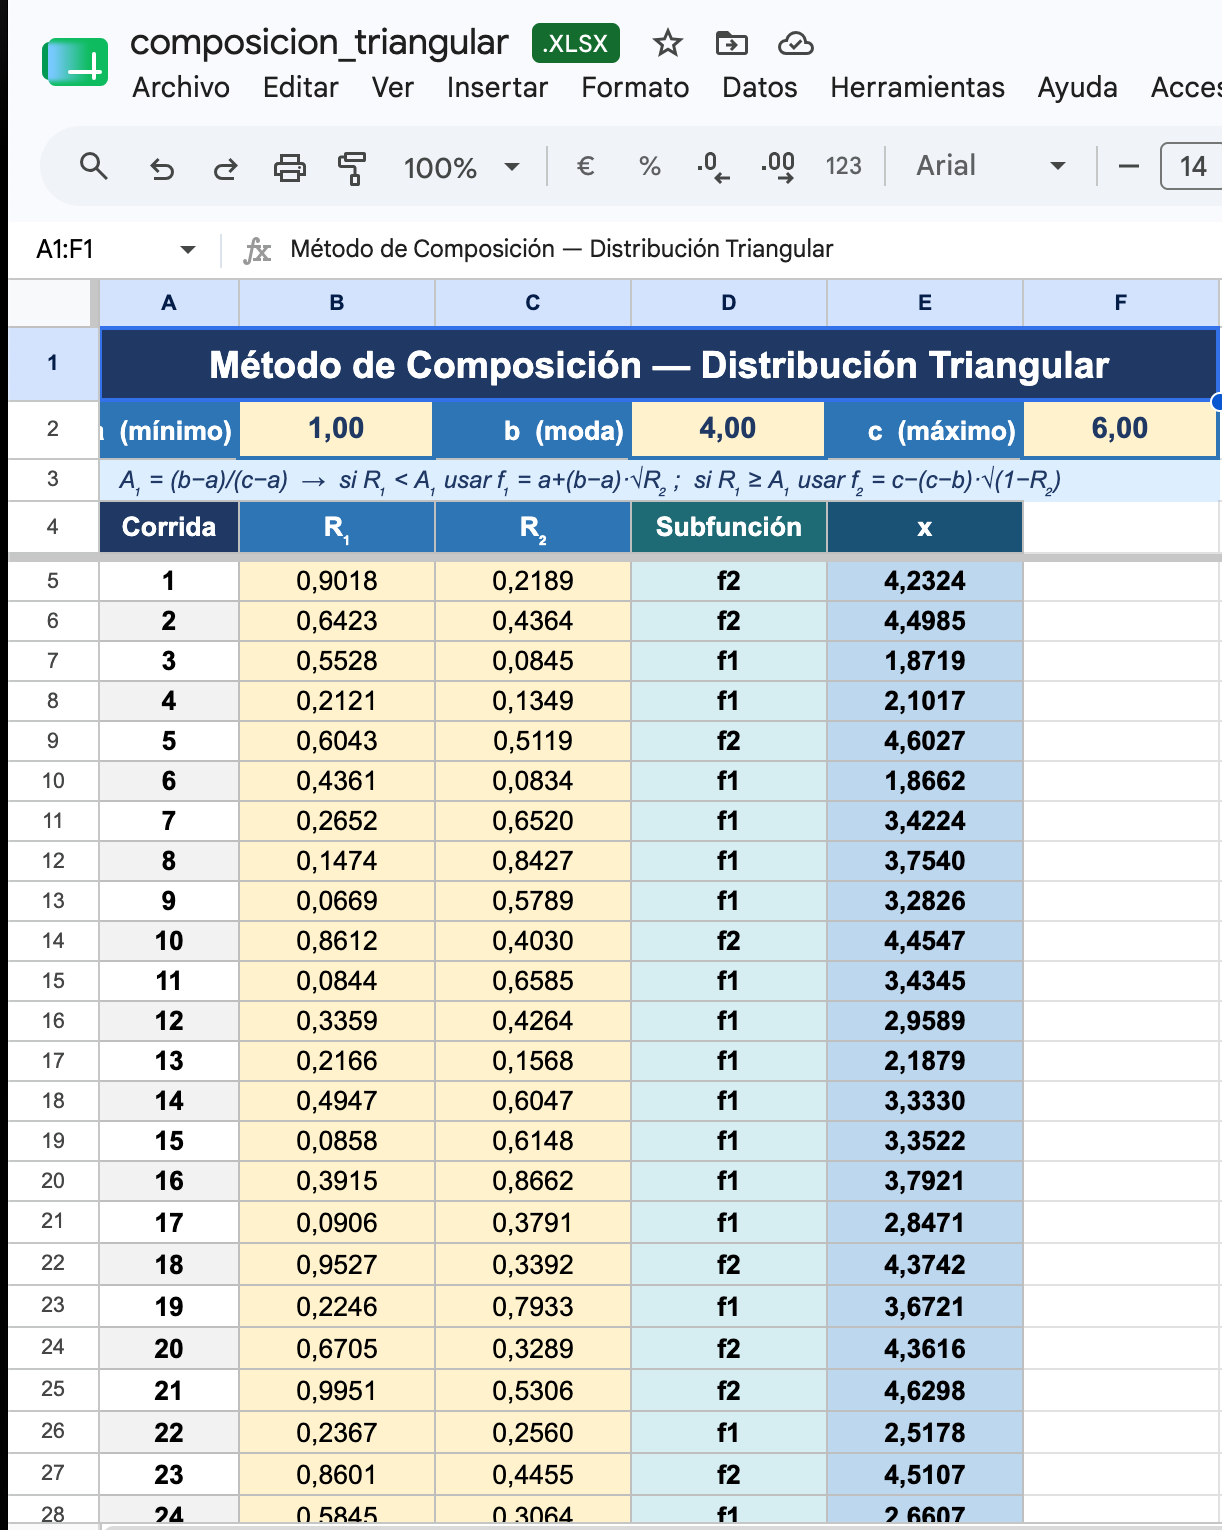
\includegraphics[width=0.9\textwidth]{capturas_excel/p2_composicion.png}
\caption{Hoja de cálculo — Composición}
\end{figure}

\subsection{Validación}

\subsubsection{\texorpdfstring{Prueba de escritorio con $n=25$}{Prueba de escritorio con n=25}}

\begin{mitabla}[H]{\texorpdfstring{Prueba de escritorio — $n=25$ corridas}{Prueba de escritorio - n=25 corridas}}
\small
\begin{tabular}{ccccc}
\toprule
Corrida & $R_1$ & $R_2$ & Sub & $x$ \\
\midrule
1  & 0,0360 & 0,8430 & $f_1$ & 3,7954 \\
2  & 0,3233 & 0,4009 & $f_1$ & 3,0830 \\
3  & 0,8452 & 0,6131 & $f_2$ & 4,9449 \\
4  & 0,8352 & 0,0089 & $f_2$ & 4,0111 \\
5  & 0,7362 & 0,4705 & $f_2$ & 4,6809 \\
6  & 0,9032 & 0,6130 & $f_2$ & 4,9448 \\
7  & 0,8695 & 0,6980 & $f_2$ & 5,1261 \\
8  & 0,4305 & 0,2852 & $f_1$ & 2,8351 \\
9  & 0,0885 & 0,3947 & $f_1$ & 3,0706 \\
10 & 0,3889 & 0,7682 & $f_1$ & 3,6912 \\
11 & 0,8191 & 0,8279 & $f_2$ & 5,4630 \\
12 & 0,4957 & 0,0343 & $f_1$ & 1,9631 \\
13 & 0,1853 & 0,6591 & $f_1$ & 3,5296 \\
14 & 0,9685 & 0,0592 & $f_2$ & 4,0751 \\
15 & 0,3201 & 0,6398 & $f_1$ & 3,4998 \\
16 & 0,6147 & 0,0361 & $f_2$ & 4,0456 \\
17 & 0,2580 & 0,0448 & $f_1$ & 2,0294 \\
18 & 0,2516 & 0,3752 & $f_1$ & 3,0314 \\
19 & 0,1156 & 0,9305 & $f_1$ & 3,9115 \\
20 & 0,6000 & 0,6125 & $f_2$ & 4,9437 \\
21 & 0,4884 & 0,2922 & $f_1$ & 2,8514 \\
22 & 0,3420 & 0,7870 & $f_1$ & 3,7178 \\
23 & 0,1244 & 0,3298 & $f_1$ & 2,9357 \\
24 & 0,9969 & 0,9364 & $f_2$ & 5,8694 \\
25 & 0,9680 & 0,3242 & $f_2$ & 4,4448 \\
\bottomrule
\end{tabular}
\end{mitabla}

$\bar{x}_{25} = 3{,}8598$

\subsubsection{\texorpdfstring{Corridas con $n \geq 50$}{Corridas con n mayor igual 50}}

\begin{mitabla}[H]{\texorpdfstring{Resumen de corridas con $n \geq 50$}{Resumen de corridas con n mayor igual 50}}
\begin{tabular}{cccc}
\toprule
$n$ & $\bar{x}$ & $x_{\min}$ & $x_{\max}$ \\
\midrule
50   & 4,2451 & 2,0906 & 5,9979 \\
100  & 4,1654 & 1,8410 & 6,0730 \\
250  & 4,0354 & 1,5589 & 6,3561 \\
500  & 3,9793 & 1,5922 & 6,3355 \\
1000 & 3,9964 & 1,7046 & 6,4485 \\
\bottomrule
\end{tabular}
\end{mitabla}

\subsection{Interpretación}

\subsubsection{Resultados}

En las 25 corridas de la prueba de escritorio, todos los valores de $x$ quedaron dentro del intervalo $[a,c]=[1{,}5,\,6{,}5]$ esperado, con media $\bar{x}_{25}=3{,}8598$, cercana al vértice $b=4$. Las corridas con $n \geq 50$ mantienen $x_{\min}$ y $x_{\max}$ dentro de $[a,c]$ y la media $\bar{x}$ se estabiliza progresivamente alrededor de $4{,}0$ conforme crece $n$.

\subsubsection{Interpretación}

Los resultados confirman que la selección de subfunción mediante $R_1$ y la aplicación de Transformada Inversa con $R_2$ generan correctamente valores de $x$ según la distribución triangular: la media se aproxima al vértice $b$ (moda de la triangular) y ningún valor generado cae fuera de $[a,c]$, lo cual es consistente con el modelo teórico planteado en la propuesta de solución.

\subsection{Conclusión}

El método de Composición permitió dividir la función triangular en dos subfunciones resueltas cada una por Transformada Inversa, seleccionadas mediante $R_1$ según la proporción de subáreas $A_1$ y $A_2$. La validación con prueba de escritorio (n=25 y $n \geq 50$) y la implementación en Java y Excel confirman que el modelo reproduce correctamente la distribución triangular esperada.
